\subsection{Simulación del proceso evolutivo}
La simulación del proceso evolutivo del mosquito del Aedes aegypti, presentado previamente en la
\secref{sec:cap4-simulador-proceso-evolutivo}, es el encargado de simular los efectos temperatura
en los siguientes eventos : eclosión de huevos, mortalidad de larvas, emergencia de pupas, muerte
de pupas, emergencia de adultos, muerte de adultos, ovipostura y dispersión de los adultos
(\figref{fig:cap-5-proceso-evolutivo}).

\begin{figure}
\centering
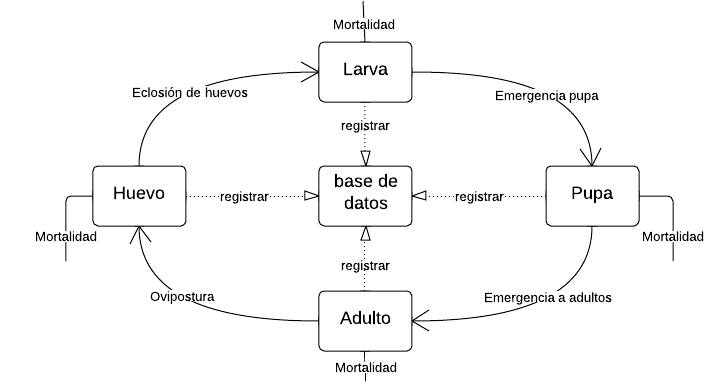
\includegraphics[width=0.8\textwidth]{capitulo-5/graphics/proceso-evolutivo.png}
\caption{\label{fig:cap-5-proceso-evolutivo} Eventos del simulador del proceso evolutivo.}
\end{figure}

La población inicial es obtenida mediante la cantidad de larvas observadas en los puntos de
control que corresponden a la muestra utilizada para el estudio. Por cada larva observada,
en un punto de control ubicado en las coordenadas geográficas, $(x, y)$, se inicializa un individuo
con las mismas coordenadas del punto de control de origen.

Las efectos de la temperatura, $k_{i}$, en cada individuo, $m_{j}$, son registrados mediante un
proceso que se encarga de almacenar, en una base de datos, la información correspondiente, de cada
$m_{j}$, para su posterior análisis.
